\subsection{Problem 4.5. Tie-in Sale Marketing Action}

\begin{quote}Once a year GTC offers a special sale. This year, one is thinking of a ``tie-in'' sale
action. A tie-in sale is a sale where the customer can obtain the desired good (tying
good) only if he/she agrees to purchase a different good (tied good). It is decided that
the tie-in sale should include two products from two separate groups of purchasable
articles. The customer has to choose one of ten different cell phones, and gets one
other product for free. The cell phones and the other products are listed in Table \ref{equip}.\end{quote}

\begin{table}[H]
	\centering
	\caption{Equipment types}
	\begin{tabular}{l||l}\hline
Cell phone type & Other product \\ \hline
GT I & Call bundle (100 min.) \\
GT II & Call bundle (200 min.) \\
GT III & Call bundle (300 min.) \\
GT IV & Call bundle (400 min.) \\
GT V & Extra Li-Ion Battery \\
GT VI & LED Flashing Keypad \\
GT VII & In-Car Charger \\
GT VIII & Belt-Clip Holster \\
GT IX & Handsfree Headset \\
GT X & USB Data Cable\\ \hline
	\end{tabular}
	\label{equip}
\end{table}

\begin{quote}So, GTC sells a cell phone together with one of the ten other products. The ten
cell phones are the tying goods, and the other products are the tied goods. Since the
other products stay, of course, available for normal sale, it is assumed that the sales
of the other products are not influenced by this action.
Based on previous actions, GTC has made an estimation of the short-term sales
increase of the phones, when combined with an other product. These estimates are
given in Table \ref{inc}. For example, GT I combined with Belt-Clip Holster, would yield
an estimated short-term sales increase of GT I of 31\%.\end{quote}

\begin{table}[H]
	\centering
	\caption{Estimates of short-term sales increase of equipment (in \%)}
	\begin{tabular}{c|*{10}c}\hline
	\multirow{2}{*}{} & \multicolumn{10}{|c}{GT} \\ \cline{2-11}
	&I&II&III&IV&V&VI&VII&VIII&IX&X\\ \hline
Call bundle (100 min.)&15&9&11&9&5&10&7&7&8&13\\ 
Call bundle (200 min.)&18&10&13&7&16&11&15&10&7&5\\ 
Call bundle (300 min.)&18&11&14&18&9&11&10&11&7&15\\ 
Call bundle (400 min.)&18&15&15&19&13&15&13&9&10&10\\ 
Extra Li-Ion Battery&20&20&18&22&18&20&17&19&13&15\\ 
LED Flashing Keypad&28&20&18&25&21&13&16&21&13&19\\ 
In-Car Charger&28&24&30&19&19&21&24&13&16&18\\ 
Belt-Clip Holster&31&34&31&29&23&24&21&21&23&16\\ 
Handsfree Headset&35&34&34&30&30&22&27&21&17&16\\ 
USB Data Cable&43&38&38&32&33&24&24&27&23&17\\
\hline
	\end{tabular}
	\label{inc}
\end{table}

\begin{table}[H]
	\centering
	\caption{Purchase and selling price of equipment (in \texteuro)}
	\begin{tabular}{l|cc}\hline
	Product & Purchase price & Selling price \\ \hline
Cell phone type & & \\ \cline{1-1}
GT I&100&300\\ 
GT II&110&330\\ 
GT III&120&360\\ 
GT IV&125&400\\ 
GT V&150&425\\ 
GT VI&160&480\\ 
GT VII&175&500\\ 
GT VIII&200&550\\ 
GT IX&250&600\\ 
GT X&300&700\\ \hline\hline
Other product & & \\ \hline
Call bundle (100 min.)&10&25\\ 
Call bundle (200 min.)&15&40\\ 
Call bundle (300 min.)&20&50\\ 
Call bundle (400 min.)&25&60\\ 
Extra Li-Ion Battery&30&75\\ 
LED Flashing Keypad&35&90\\ 
In-Car Charger&40&100\\ 
Belt-Clip Holster&45&125\\ 
Handsfree Headset&50&150\\ 
USB DataCable&55&160	\\ \hline
	\end{tabular}
	\label{price}
\end{table}

\begin{quote}The problem for GTC is to combine cell phones with other products, one cell
phone to one other product, and vice versa, such as to maximize total profit.\end{quote}

	\paragraph{}
	First of all let's explain how we computed prices/profits of the products and their combinations. The profit of the single phone/other product is evaluated as the difference between its selling price and purchase price taken from Table \ref{price}. The profit of the combination of the cell phone and other product is equal to the sum of individual profits of these two items taken from Table \ref{price} increased by corresponding number of per cent taken from the Table \ref{inc}.

\begin{enumerate}[(a)]
\setcounter{enumi}{1}
\item\begin{quote}By inspection, how would you combine the products? What is the rationale behind
your solution procedure?\end{quote}

	\paragraph{}
	The immediate thought would be to combine greedily. We will repeat the following procedure number of products times --- 10 times. On each iteration we will choose the best (the most profitable) pair of cell phone and other product among currently unpaired phones and products. The idea behind this approach is that on every iteration we choose the best available variant thus maximizing our immediate profit as if the already matched products do not exist (they are sold, for example). The greedy approach is attractive because of its simplicity but it doesn't necessary lead to an optimal solution. The assignment is shown in Table \ref{greedy-5-b}. The total profit equals \texteuro4,167.00.

\begin{table}[H]
	\centering
	\caption{Greedy assignment of cell phone -- other product pairs}
	\begin{tabular}{|c|c|c|}\hline
Cell phone type & Other product & Price (including short-term increase) \\ \hline
GT I & Call bundle (100 min.) & 247.25 \\
GT II & Call bundle (200 min.) & 269.50 \\
GT III & Call bundle (300 min.) & 307.80 \\
GT IV & LED Flashing Keypad & 412.50 \\
GT V & Call bundle (400 min.) & 350.30 \\
GT VI & Extra Li-Ion Battery & 438.00 \\
GT VII & In-Car Charger & 477.40 \\
GT VIII & Handsfree Headset & 544.50 \\
GT IX & Belt-Clip Holster & 528.90 \\
GT X & USB Data Cable & 590.85 \\
\hline
	\end{tabular}
	\label{greedy-5-b}
\end{table}

\item\begin{quote}Set up a model to solve the problem. Determine and analyze your optimal solution.\end{quote}

	\paragraph{}
	Let's consider a complete bipartite graph $G=(S,T,E)$ with set of vertices $S$ corresponding to other products and set of vertices $T$ corresponding to cell phones ($|T|=|C|=10$). Between each pair of vertices where one corresponds to the $i$-th product and other --- to the $j$-th cell phone there is an edge with an assigned weight $w_{ij}$ that is equal to the profit that we gain when combining product $i$ with cell phone $j$. The cost matrix of this graph $W=\{w_{ij}\}$ is shown in Table \ref{graph-5-c}. The rows correspond to other products and columns correspond to cell phones.

\begin{table}[H]
	\centering
	\caption{Cost matrix $W$ for an optimal assignment problem of cell phones to other products}
	\begin{tabular}{|*{11}{c|}}\hline
Products\textbackslash GT & I & II & III & IV & V & VI & VII & VIII & IX & X\\\hline
Call bundle (100 min.) & 247.25  & 256.15  & 283.05  & 316.10  & 304.50  & 368.50  & 363.80  & 390.55  & 394.20  & 468.95 \\ \hline
Call bundle (200 min.) & 265.50  & 269.50  & 299.45  & 321.00  & 348.00  & 382.95  & 402.50  & 412.50  & 401.25  & 446.25 \\ \hline
Call bundle (300 min.) & 271.40  & 277.50  & 307.80  & 359.90  & 332.45  & 388.50  & 390.50  & 421.80  & 406.60  & 494.50 \\ \hline
Call bundle (400 min.) & 277.30  & 293.25  & 316.25  & 368.90  & 350.30  & 408.25  & 406.80  & 419.65  & 423.50  & 478.50 \\ \hline
Extra Li-Ion Battery & 294.00  & 318.00  & 336.30  & 390.40  & 377.60  & 438.00  & 432.90  & 470.05  & 446.35  & 511.75 \\ \hline
LED Flashing Keypad & 326.40  & 330.00  & 348.10  & 412.50  & 399.30  & 423.75  & 440.80  & 490.05  & 457.65  & 541.45 \\ \hline
In-Car Charger & 332.80  & 347.20  & 390.00  & 398.65  & 398.65  & 459.80  & 477.40  & 463.30  & 475.60  & 542.80 \\ \hline
Belt-Clip Holster & 366.80  & 402.00  & 419.20  & 457.95  & 436.65  & 496.00  & 490.05  & 520.30  & 528.90  & 556.80 \\ \hline
Handsfree Headset & 405.00  & 428.80  & 455.60  & 487.50  & 487.50  & 512.40  & 539.75  & 544.50  & 526.50  & 580.00 \\ \hline
USB Data Cable & 436.15  & 448.50  & 476.10  & 501.60  & 505.40  & 527.00  & 533.20  & 577.85  & 559.65  & 590.85 \\ \hline
	\end{tabular}
	\label{graph-5-c}
\end{table}
	
	\paragraph{}
	The optimization problem for an optimal assignment can be stated as follows.
$$
	\textbf{Maximize}
$$
$$
	z = \sum\limits_{i\in S, j\in T} w_{ij}x_{ij}
$$
$$
	\textbf{Subject to}
$$
$$
	\sum\limits_{j\in T} x_{ij} \leq 1 \ \text{for each }i\in S
$$
$$
	x_{ij} \geq 0 \ \text{for each }i\in S,\  j\in T
$$

	\paragraph{}
	Indeed, our task is to combine other products and cell phones in pairs in such a way that every product and every cell phone is present in exactly one pair and the sum of profits of all the pairs is maximized. The stated optimization problem is equivalent to the Assignment Problem --- problem of finding the maximum weight perfect matching in a complete bipartite graph. This problem can be effectively solved using Hungarian algorithm with matrix $W$ as an input cost matrix. The optimal assignment is shown in the Table \ref{hungarian-5-c}. The total profit equals \texteuro4,304.80 which is greater than the one obtained using greedy strategy.

\begin{table}[H]
	\centering
	\caption{Optimal assignment problem of cell phones to other products}
	\begin{tabular}{|c|c|c|}\hline
Cell phone type & Other product & Price (including short-term increase) \\ \hline
GT I & USB Data Cable & 436.15 \\
GT II & Belt-Clip Holster & 402.00 \\
GT III & Handsfree Headset & 455.60 \\
GT IV & Call bundle (400 min.) & 368.90 \\
GT V & Call bundle (200 min.) & 348.00 \\
GT VI & Extra Li-Ion Battery & 438.00 \\
GT VII & In-Car Charger & 477.40 \\
GT VIII & LED Flashing Keypad & 490.05 \\
GT IX & Call bundle (100 min.) & 394.20 \\
GT X & Call bundle (300 min.) & 494.50 \\
\hline
	\end{tabular}
	\label{hungarian-5-c}
\end{table}

\setcounter{enumi}{0}
\item\begin{quote}Determine the minimum required short-term sales increase that makes the combination
GT I with Extra Li-Ion Battery profitable, in terms of percentage. The
purchase prices and selling prices are listed in Table \ref{price}.\end{quote}

	\paragraph{}
	Let's evaluate the perturbation function of the short-term sales increase of the combination GT I with Extra Li-Ion Battery from Table \ref{inc}. We will iterate through possible values of this parameter starting from the initial one and evaluate the optimal assignment as in part (b) until it will be profitable to include pair GT I -- Extra Li-Ion Battery in the optimal solution. The perturbation function is given in Table \ref{tol-5-a}. We can observe that the minimum required increase in the considered parameter that makes the combination GT I with Extra Li-Ion Battery profitable (makes this pair appear in a optimal solution) is equal to 10. This increase is upper tolerance of this parameter by definition.

\begin{table}[H]
	\centering
	\caption{Perturbation function of the sales increase when combining GT I with Extra Li-Ion Battery}
	\begin{tabular}{|c|c|c|}\hline
	Value of the parameter & Cost of the optimal solution & Product GT I is paired with \\ \hline
20 & 4304.80 & USB Data Cable \\
21 & 4304.80 & USB Data Cable \\
22 & 4304.80 & USB Data Cable \\
23 & 4304.80 & USB Data Cable \\
24 & 4304.80 & USB Data Cable \\
25 & 4304.80 & USB Data Cable \\
26 & 4304.80 & USB Data Cable \\
27 & 4304.80 & USB Data Cable \\
28 & 4304.80 & USB Data Cable \\
29 & 4304.80 & USB Data Cable \\
30 & 4304.85 & Extra Li-Ion Battery \\
	\hline
	\end{tabular}
	\label{tol-5-a}
\end{table}

\setcounter{enumi}{3}
\item\begin{quote}For the model used in part (c), draw and analyze the perturbation function of the
coefficient representing the additional net sales of the combination GT IV with
Call Bundle of 400 minutes.\end{quote}

	\paragraph{}
	To draw the perturbation function we'll iterate through possible values of the additional net sales of the combination GT IV with
Call Bundle of 400 minutes and calculate the profit of an optimal assignment using Hungarian algorithm. The perturbation function is shown in the Figure \ref{perturbation-5-d}.

\begin{figure}[H]
	\centering
	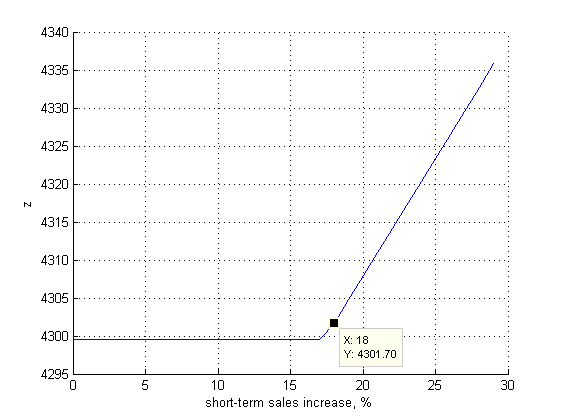
\includegraphics[scale=1]{./img/perturbation-5-d.png}
	\caption{Perturbation function of the Assignment Problem of the additional net sales of the combination GT IV with Call Bundle of 400 minutes}
	\label{perturbation-5-d}
\end{figure}

	\paragraph{}
	From the Figure \ref{perturbation-5-d} we can see that starting from value equal to 18 GT IV is combined with Call bundle (400 min.) in an optimal solution. The lower values of the parameter lead to exclusion of this pair from an optimal solution. It's clear that decreasing this value below 17 won't return this combination to the solution and increasing after 18 won't move this pair from the optimal assignment. Knowing perturbation function we are able to calculate the lower tolerance of this parameter --- the maximal decrease that leaves the considered combination in the optimal solution. Upper tolerance of $w_{2,14}$ equals $1177 - 1163 = 136 - 122 = 14$.



\end{enumerate}